In HDDs when the OS addresses a sector, it gets the exact same sector from the drive, while in SSDs, the FTL manages the way in which a logical address requested by the OS is mapped into the respective physical block address on memory chips.\\
The underlying mapping is completely transparent and can be modified by the FTL at any time for any reason. The FTL may move data around or blank data even if the OS is not running.
\section{Can we bypass the FTL?}
    We don't know hot the FTL works, it is proprietary information of the company which produces it. We need to bypass it.\\
    It is not possible by software, it is in theory possible by directly reading the memory chips, using a custom setup built to interact with flash memory chips using an FPGA. This is in any case:
    \begin{itemize}
        \item Extremely time and money consuming: there is the need to buy and manage custom hardware, reverse-engineering of the FTL data management.
        \item Non repeatable: the operation of physically extracting the memory chips may be destructive or alterating.
    \end{itemize}
    Mobile devices work in a similar way, so they have the same problems.
\section{Challenges in black box analysis and goals}
    \subsection{An unclear picture}
        Most of our recovery of deleted files works because of leftovers on the drive. If the chip trims the drive, the leftovers are no more there: we need to know how fast trimming happens. Since this is performed by the FTL chip, it is performed when the drive is turned on, even if the drive is not connected to any computer. Write blockers don't work too.\\
        USB sticks has the same fastidious characteristic. Notice that this causes the hashes to be different everytime.\\
        Carving don't woek at all on SSDs.\\
        What the professors did was to test different SSDs to determine what was possible to do, and which was the impact of FTL on the use of black-box tools.
    \subsection{Testing methodology}
        They tested for:
        \begin{itemize}
            \item Trimming: negative impact on forensics as data persistence is reduced, it happens even with a write blocker. They wanted to determine the percentage of erased blocks and how fast.
            \item Garbage collection: they wanted to determine whether it is employed by the SSD under examination.
            \item Erasing Patterns: they found out that particular behaviors were shown by some SSDs when using trimming.
            \item Compression: to verify if it was active
            \item Wear leveling
            \item Files recoverability 
        \end{itemize}
    \subsection{Test drives}
        They used three different test drives, equipped with a small amount of DRAM-based cache memory to reduce physical writes, which was disabled.
    \subsection{Trimming}
        \begin{figure}[ht!]
            \centering
            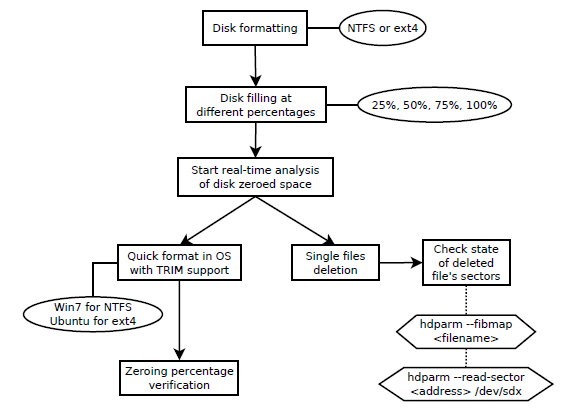
\includegraphics[width=0.8\linewidth]{trim.png}
            \caption{trimming test flow}
        \end{figure}
        Their results:
        \begin{itemize}
            \item If trim is present and active, it activates in 1-10 seconds 
            \item NTFS wiped the disk in less than 10 seconds 
            \item ext4 erased the disk in about 15 seconds when formatting, some drives did not erase on delete, some only when unmounting.
        \end{itemize}
        Consider that nowadays most of the filesystems support SSDs, so they will work correctly. But it may be useful to check for any remainance.
    \subsection{Garbage Collection}
        \begin{figure}[ht!]
            \centering
            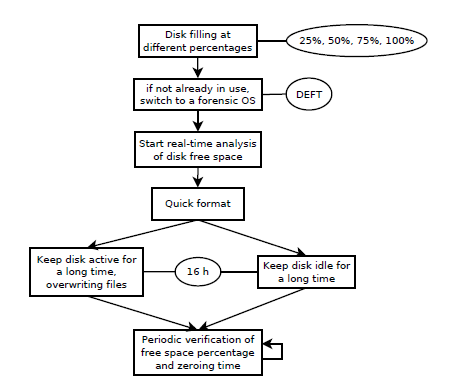
\includegraphics[width=0.8\linewidth]{garbage.png}
            \caption{garbage collection test flow}
        \end{figure}
        In their tests, none of the SSDs performed garbage collection, even when trying to repeat a documented experiment with the help of the author of that experiment.
    \subsection{Erasing Patterns}
        \begin{figure}[ht!]
            \centering
            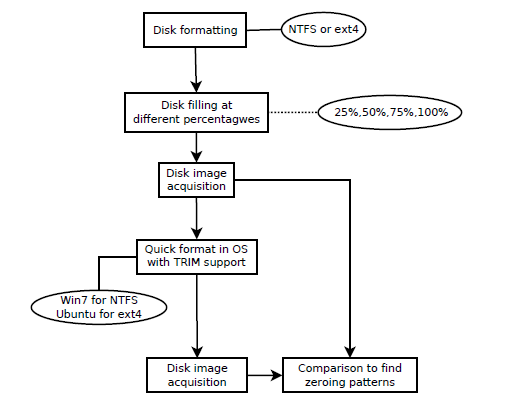
\includegraphics[width=0.8\linewidth]{patterns.png}
            \caption{erasing patterns test flow}
        \end{figure}
        They found out that certain SSD controllers may exhibit unexpected trimming patterns, leaving some parts \textit{more recoverable} than others. What the professor thinks is that the drive could be faulty, but this is important to check then, faulty drives may still keep data.
    \subsection{Compression}
        \begin{figure}[ht!]
            \centering
            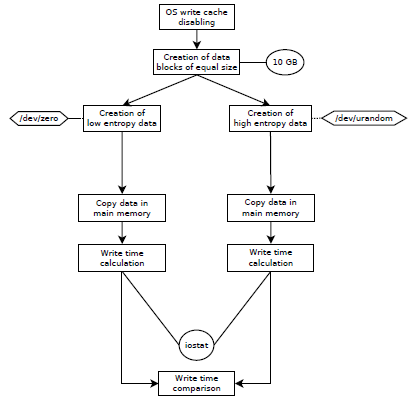
\includegraphics[width=0.8\linewidth]{compression.png}
            \caption{compression test flow}
        \end{figure}
        They found out that some drives had less data transferred when transfering the same file, thus compression.
    \subsection{Wear Leveling}
        \begin{figure}[ht!]
            \centering
            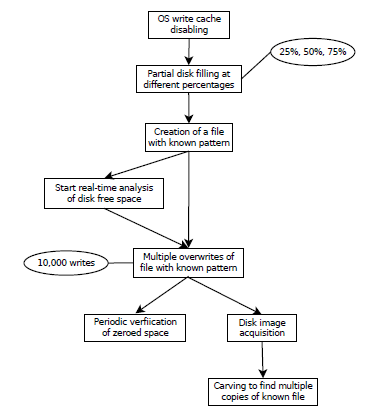
\includegraphics[width=0.8\linewidth]{wearleveling.png}
            \caption{wear leveling test flow}
        \end{figure}
        They wanted to find if more copies of the same data were created while doing wear leveling. They weren't.
    \subsection{Files Recoverability}
        \begin{figure}[ht!]
            \centering
            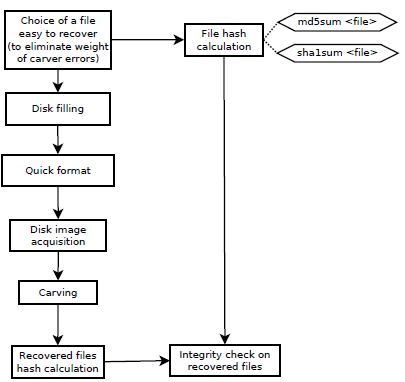
\includegraphics[width=0.8\linewidth]{recoverability.png}
            \caption{files recoverability test flow}
        \end{figure}
        Only the drive which presented trimming had recoverable files.